
% This LaTeX was auto-generated from MATLAB code.
% To make changes, update the MATLAB code and republish this document.

\documentclass{article}
\usepackage{graphicx}
\usepackage{color}

\sloppy
\definecolor{lightgray}{gray}{0.5}
\setlength{\parindent}{0pt}

\begin{document}

    
    




\subsection*{Constants}

\begin{verbatim}
Q1_0 = 0.125e-6;
c0 = 120;
\end{verbatim}


\subsection*{Equations portion}

\begin{verbatim}
c1_0(1,1:200) = c0;

fstarL = linspace(0,1.5e-5,200);
alpha = fstarL/(Q1_0*c0);

c2_0 = c0*(1-alpha).*exp(alpha);

%Total flux in and out of the loop
flux_in = Q1_0 * c0;
flux_out = flux_in*(1-alpha);
flux_in(1,1:200) = flux_in;
\end{verbatim}


\subsection*{Plotting}

\begin{verbatim}
close all
figure
hold on; box on;
axis([0, 1.6e-5, 0, 150])

plot(fstarL,c1_0,'k--')
plot(fstarL,c2_0,'k')
%line([0,1.6e-5],[120,120],'LineStyle','--','Color','k')
legend('c_1(0)','c_2(0)','Location','SouthWest')

xlabel('Total pumping rate, f^*_{Na}L (mEq/min)')
ylabel('Concentration (mEq/L)')

hold off

figure
hold on; box on;

plot(fstarL,flux_in,'k--')
plot(fstarL,flux_out,'k')

legend('flux in','flux out','Location','SouthWest')

xlabel('Total pumping rate, f^*_{Na}L (mEq/min)')
ylabel('Total sodium flux (mEq/min)')

hold off
\end{verbatim}

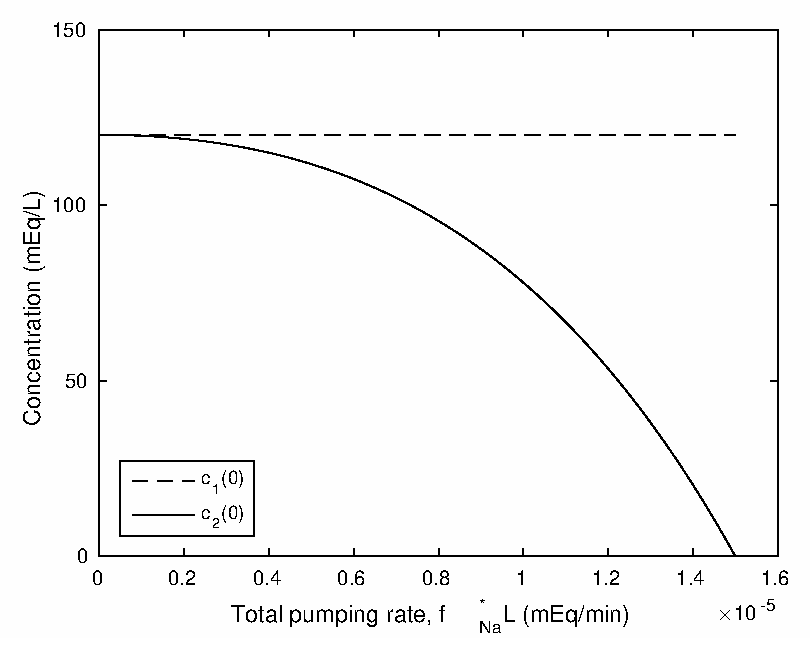
\includegraphics [width=4in]{Q1_01.eps}

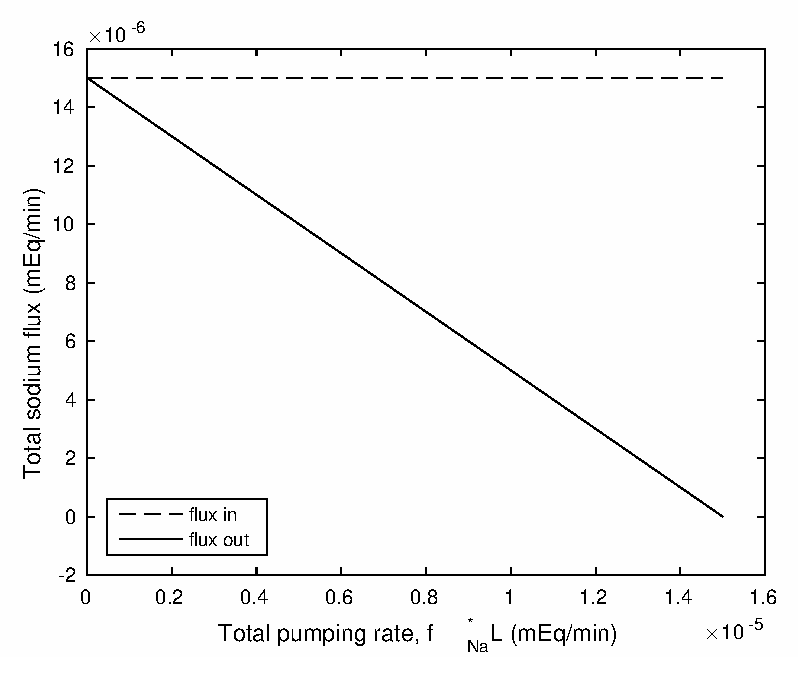
\includegraphics [width=4in]{Q1_02.eps}



\end{document}
    
